\documentclass[11pt]{article}
\usepackage{booktabs}
\usepackage{natbib}
\usepackage{fullpage}
\usepackage{fancyhdr}

\usepackage{amsmath}
\usepackage{amssymb}
\usepackage{url}

\usepackage{listings}
\usepackage{color}
\lstset{%
        basicstyle=\footnotesize\ttfamily,
        showspaces=false,
        showstringspaces=false,
        tabsize=2,
        breaklines=false,
        breakatwhitespace=true,
        identifierstyle=\ttfamily,
        keywordstyle=\color[rgb]{0,0,1},
        commentstyle=\color[rgb]{0.133,0.545,0.133},
        stringstyle=\color[rgb]{0.627,0.126,0.941},
    }

\usepackage{graphicx}
\usepackage{qtree}

% header
\fancyhead{}
\fancyfoot{}
\fancyfoot[C]{\thepage}
\fancyhead[R]{Daniel Foreman-Mackey}
\fancyhead[L]{Statistical Natural Language Processing --- Homework 5}
\pagestyle{fancy}
\setlength{\headsep}{10pt}
\setlength{\headheight}{20pt}

% shortcuts
\newcommand{\Eq}[1]{Equation (\ref{eq:#1})}
\newcommand{\eq}[1]{Equation (\ref{eq:#1})}
\newcommand{\eqlabel}[1]{\label{eq:#1}}
\newcommand{\Fig}[1]{Figure~\ref{fig:#1}}
\newcommand{\fig}[1]{Figure~\ref{fig:#1}}
\newcommand{\figlabel}[1]{\label{fig:#1}}

\newcommand{\etal}{\emph{et al.}}

\newcommand{\pr}[1]{\ensuremath{p\left (#1 \right )}}
\newcommand{\lk}[1]{\ensuremath{\mathcal{L} \left ( #1 \right )}}
\newcommand{\bvec}[1]{\ensuremath{\boldsymbol{#1}}}
\newcommand{\dd}{\ensuremath{\, \mathrm{d}}}
\newcommand{\normal}[2]{\ensuremath{\mathcal{N} \left ( #1; #2 \right ) }}
\newcommand{\T}{^\mathrm{T}}

\newcommand{\data}{\mathcal{D}}
\newcommand{\code}[1]{{\sffamily #1}}
\DeclareMathOperator*{\argmax}{arg\,max}


\begin{document}

For this assignment, I leaded the data and extracted the probabilistic grammar
using Python and then implemented my CKY algorithm in C (because I couldn't
come up with a way of doing it without loops).
I used the NLTK\footnote{\url{http://nltk.org}} module for I/O because it
includes methods for reading Penn Treebank-style tagged trees.
I implemented the rest of the code by hand.
As I will show below, the training step of my algorithm is quite slow but my
final inference algorithm can parse a 20 word sentence in approximately XXXX
seconds.
All of the code that I used for this assignment and the source code for this
document is available on GitHub at \url{https://github.com/dfm/nlp} in the
\code{hw5} directory.

\section{Introduction}

In this assignment, I'm are solving the syntactic parsing problem.
Given a sentence, I would like to infer the syntactic tree structure with
maximum probability under an empirical probabilistic context-free grammar.
The grammar consists of lexical rules and non-terminal emission rules.
The lexical rules have the form
\begin{eqnarray}
p(\mathrm{POS} \to \mathrm{word}) &=& p(\mathrm{word}\,|\,\mathrm{POS})
\end{eqnarray}
where \code{POS} is a part-of-speech tag and \code{word} is a word (that may
or may not be in the known vocabulary).
I estimated these probabilities from the training data using the same method
as the provided Java framework.
The non-lexical rules can be unaries or binaries estimated as
\begin{eqnarray}
p(\mathrm{A} \to \mathrm{B}) &=& p(\mathrm{B}\,|\,\mathrm{A}) \\
                             &=& \frac{f(\mathrm{A}\to\mathrm{B})}
                                 {\sum_\mathrm{X} f(\mathrm{A}\to\mathrm{X})}
\end{eqnarray}
or
\begin{eqnarray}
p(\mathrm{A} \to \mathrm{B\,C}) &=& p(\mathrm{B},\,\mathrm{C}\,|\,\mathrm{A}) \\
                                &=& \frac{f(\mathrm{A}\to\mathrm{B\,C})}
                                    {\sum_\mathrm{X} f(\mathrm{A}\to\mathrm{X})}
\end{eqnarray}
respectively, where the sum over X includes both unary and binary emissions.

\section{Tree normalization}

Since the model that I'm using only includes unary and binary rules, we need
to normalize the training trees before building the grammar.
The standard normalization form is ``Chomsky normal form'' and the
normalization algorithm is defined by a few simple rules and choices.
In particular, an approximate normalization is normally a better choice than
the exact form because the grammar will generalize more robustly.
It is easiest to describe this algorithm by showning an example.
Tree~\ref{eq:normalization}a below shows a hypothetical tagged syntactic tree
with more general rules than just unaries and binaries.
A possible lossless---or infinite-order---normalization is shown in
tree~\ref{eq:normalization}b.
In this representation, the node subscripts indicate the names of the sibling
nodes in the original tree and the superscripts keep track of the parents of
the normalized clique.
The default baseline normalization given in the homework is an infinite
horizontal and zeroth order vertical Markovization.
The representation of this tree in that form is given in
tree~\ref{eq:normalization}c.
A lossier but potentially more general tree is shown in
tree~\ref{eq:normalization}d.
Specifically, this last normalization a first-order vertical and
first-order horizontal Markov process.
\begin{eqnarray}\eqlabel{normalization}
&\begin{array}{cc}
\mbox{(a) reference tree} &
\mbox{(b) lossless normalization} \\
\hspace{0.3in}
\Tree [.S [.A [.B ] [.C ] [.D ] [.E ]]]
\hspace{0.3in} & \hspace{0.3in}
\Tree [.S [.A^S [.B ] [.A^S_{C,D,E} [.C ] [.A^S_{D,E} [.D ] [.E ]]]]]
\hspace{0.3in}
\end{array}& \nonumber\\
&\begin{array}{cc}
\mbox{(c) baseline normalization} &
\mbox{(d) finite-order Markovization} \\
\hspace{0.3in}
\Tree [.S [.A [.B ] [.A_{C,D,E} [.C ] [.A_{D,E} [.D ] [.E ]]]]]
\hspace{0.3in} & \hspace{0.3in}
\Tree [.S [.A^S [.B ] [.A^S_{C} [.C ] [.A^S_{D} [.D ] [.E ]]]]]
\hspace{0.3in}
\end{array}&
\end{eqnarray}

\section{Inference of tree structure}

The inference problem that we need to solve for this assignment is
\begin{eqnarray}
    G^* = \argmax_{G} p (G\,|\,\bvec{w})
\end{eqnarray}

\section{Experiments}

% \begin{figure}[htbp]
% \begin{center}
%     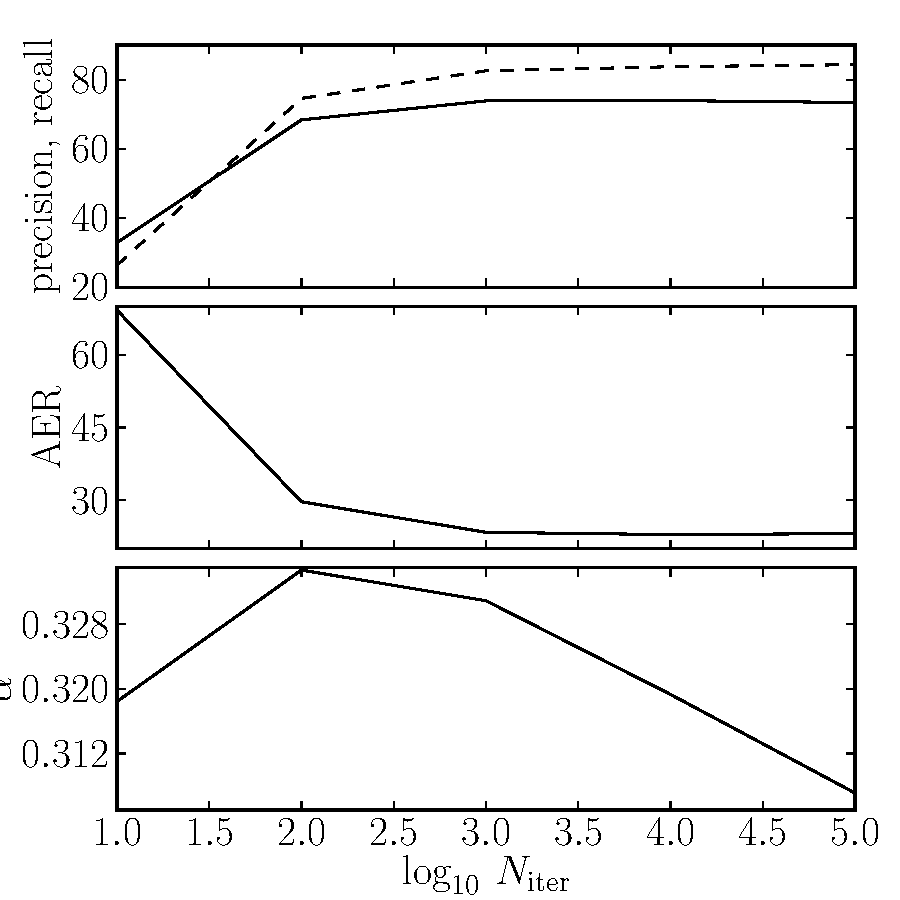
\includegraphics[width=0.5\textwidth]{model2_convergence.pdf}
% \end{center}
% \caption{%
% The same as \fig{model2-convergence} but using \emph{Model 2}.
% The bottom panel here shows the value of $\alpha$ at each step.
% \figlabel{model2-convergence}}
% \end{figure}
%
% \begin{thebibliography}{}\raggedright
%
% \bibitem[Brown \etal(1993)]{ibm}
% P.~F.~Brown, S.~A.~Della\ Pietra, V.~J.~Della\ Pietra, \& R.~L.~Mercer (1993)
% \textbf{The Mathematics of Statistical Machine Translation: Parameter
%         Estimation}, Computational Linguistics, 19, 2
%
% \end{thebibliography}

\end{document}
